\documentclass{article}

\usepackage{graphicx}
\usepackage{tikz}
\usepackage{tikzsymbols}
\usetikzlibrary{calc,patterns,shapes.geometric}
\pagestyle{empty}
\usepackage[margin=0pt]{geometry}
\geometry{papersize={14in,12in}}

\def\centerarc[#1](#2)(#3:#4:#5){\draw[#1] ($(#2)+({#5*cos(#3)},{#5*sin(#3)})$) arc (#3:#4:#5);}

\begin{document}
	\begin{figure}
		\centering
		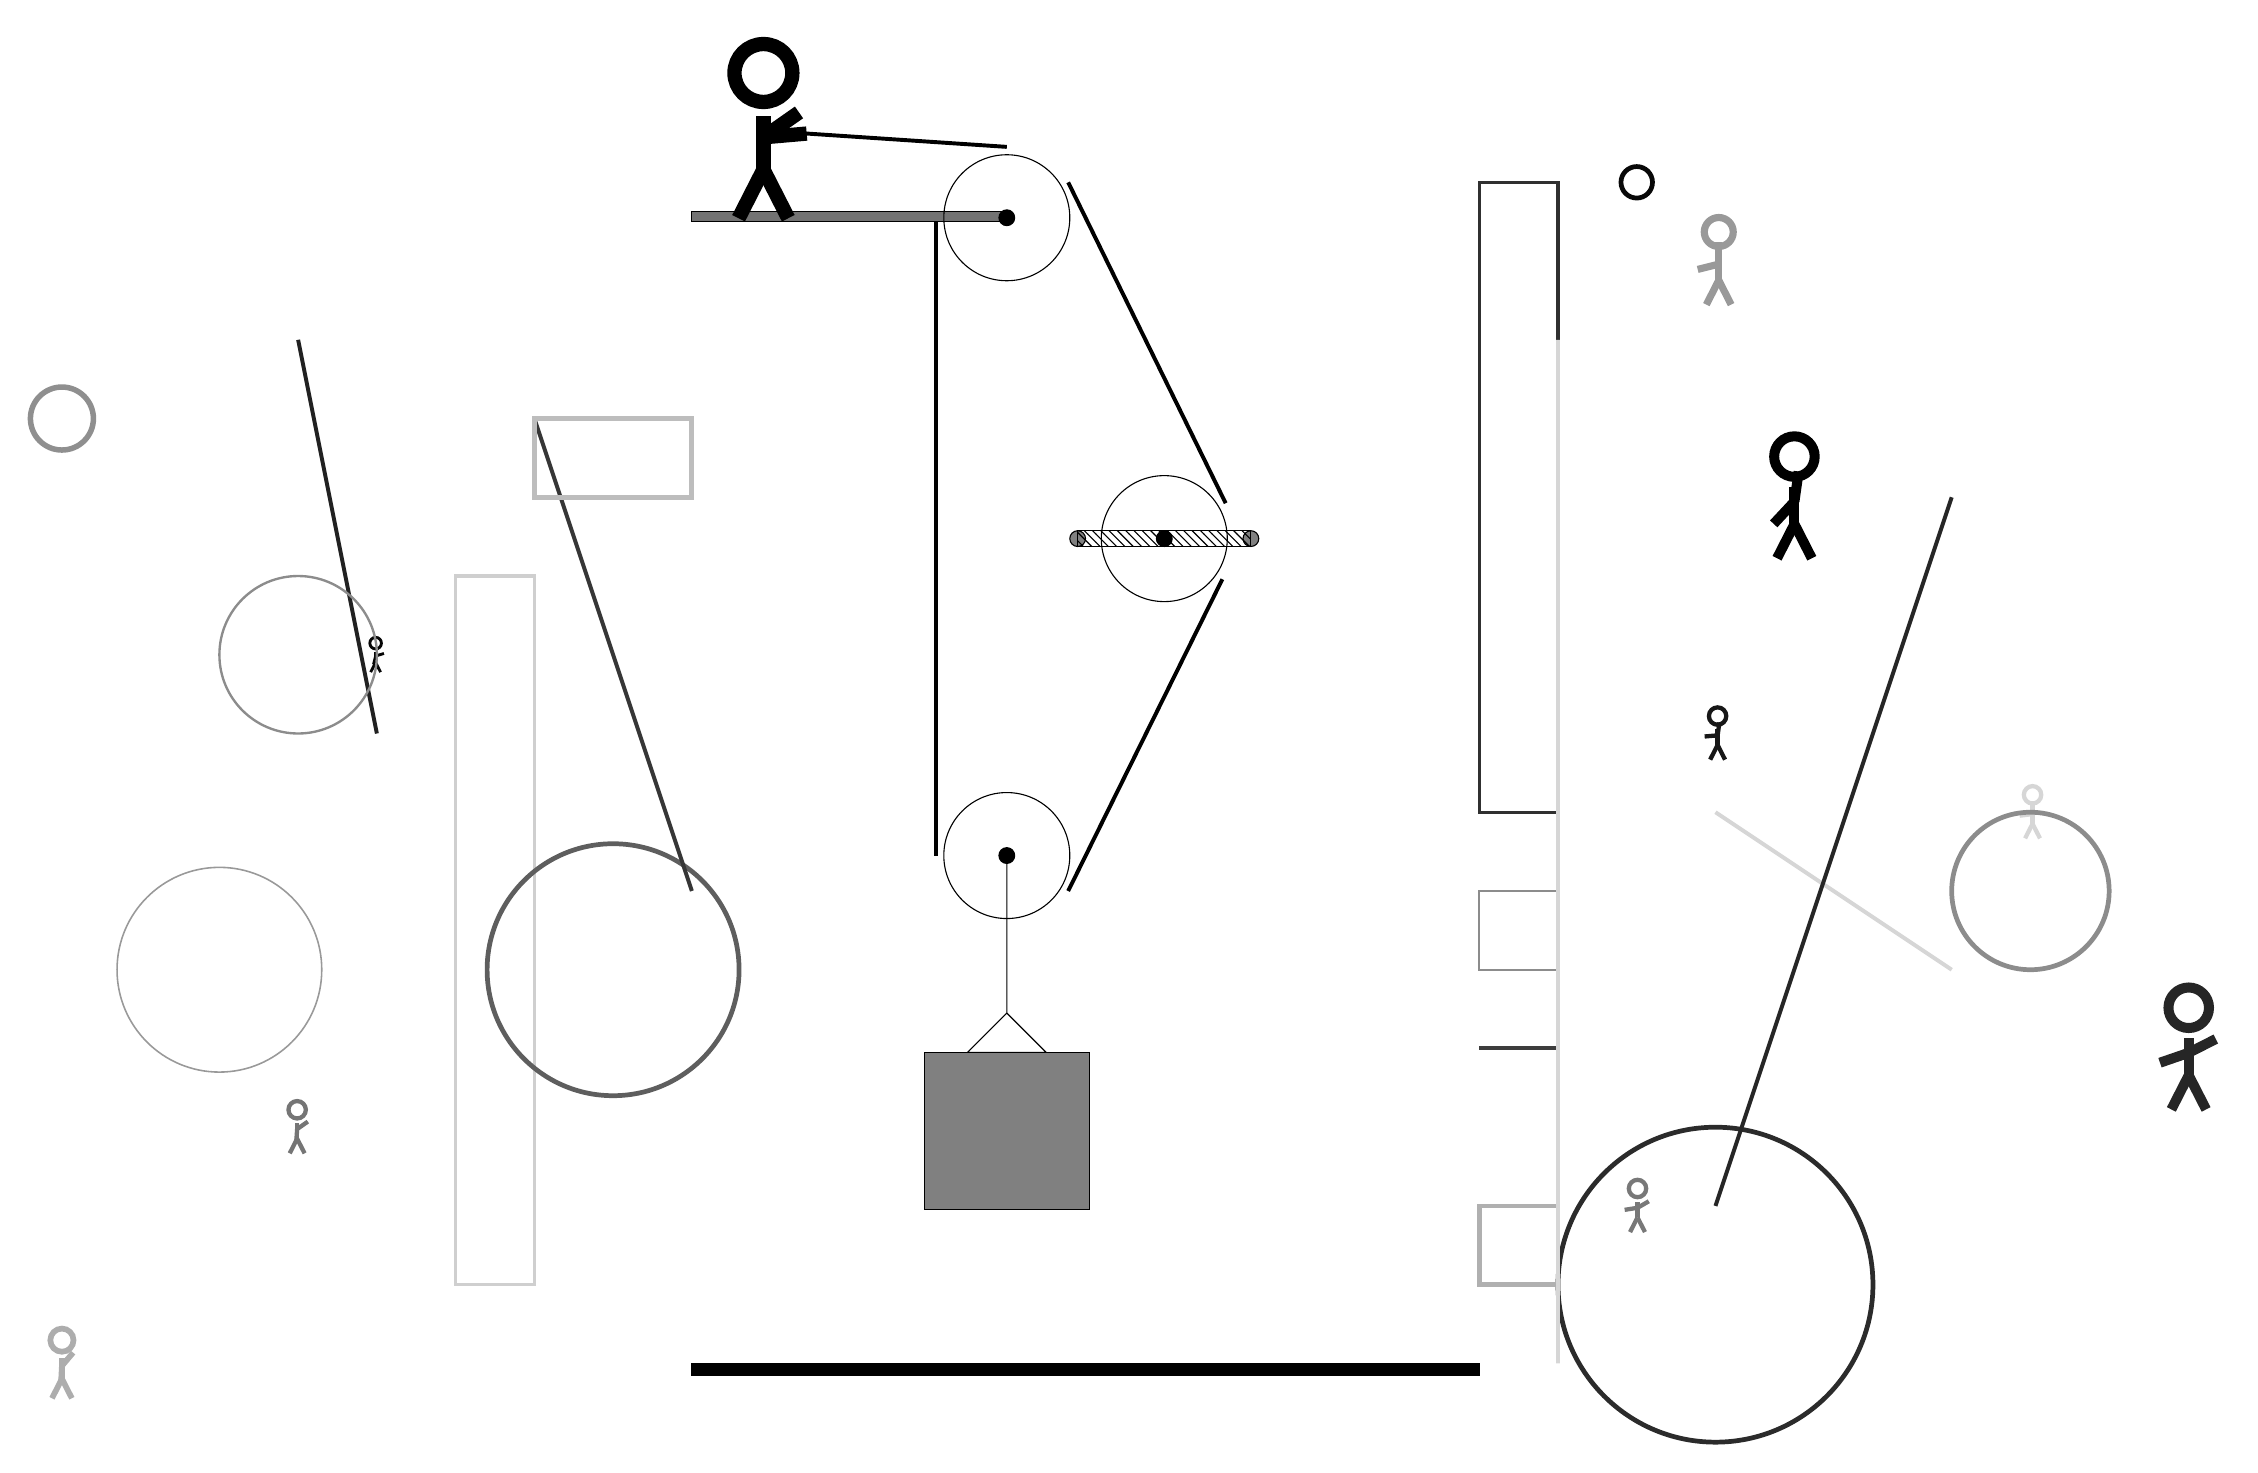
\begin{tikzpicture}
			%%%%% START %%%%%
			
			\draw[fill=black!55] (-2, 11.5) rectangle (2, 11.625);
			
			\draw (2, 3.45) circle (0.8);
			\draw[fill=black] (2, 3.45) circle (0.1);
			
			\draw (2, 11.55) circle (0.8);
			\draw[fill=black] (2, 11.55) circle (0.1);
			
			\node[line width=0.3mm, color=black!40] at (11, 11) {\Strichmaxerl[5][14][90]};
			
			\node[line width=0.5mm, color=black!53] at (10, -1) {\Strichmaxerl[3][9][30]};
			\draw[line width=0.4mm, color=black!19] (-4, -2) rectangle (-5, 7);
			\draw[line width=0.5mm, color=black!16](11, 4) -- (14, 2);
			
			\draw [line width=0.6mm, color=black!97](10, 12) circle (0.2);
			
			\node[line width=0.2mm, color=black!54] at (-7, 0) {\Strichmaxerl[3][86][35]};
			\node[line width=0.2mm, color=black!100] at (12, 8) {\Strichmaxerl[7][47][82]};
			\node[line width=0.7mm, color=black!98] at (-6, 6) {\Strichmaxerl[2][76][17]};
			\node[line width=0.7mm, color=black!32] at (-10, -3) {\Strichmaxerl[4][87][50]};
			\draw[line width=0.5mm, color=black!87](-6, 5) -- (-7, 10);
			\draw [line width=0.6mm, color=black!63](-3, 2) circle (1.6);
			
			\draw[line width=0.5mm, color=black!79](-2, 3) -- (-4, 9);
			\draw[line width=0.5mm, color=black!76](8, 1) -- (9, 1);
			
			\draw[line width=0.2mm, color=black!45] (8, 3) rectangle (9, 2);
			\node[line width=0.2mm, color=black!85] at (17, 1) {\Strichmaxerl[7][19][27]};
			\draw [line width=0.6mm, color=black!83](11, -2) circle (2.0);
			
			\draw[line width=0.5mm, color=black!85](11, -1) -- (14, 8);
			\draw[line width=0.6mm, color=black!31] (9, -1) rectangle (8, -2);
			\draw[line width=0.4mm, color=black!81] (9, 12) rectangle (8, 4);
			\draw [line width=0.2mm, color=black!40](-8, 2) circle (1.3);
			\draw [line width=0.3mm, color=black!45](-7, 6) circle (1.0);
			\node[line width=0.6mm, color=black!16] at (15, 4) {\Strichmaxerl[3][7][90]};
			\node[line width=0.6mm, color=black!91] at (11, 5) {\Strichmaxerl[3][5][82]};
			\draw [line width=0.6mm, color=black!45](15, 3) circle (1.0);
			\draw [line width=0.7mm, color=black!44](-10, 9) circle (0.4);
			\draw[line width=0.6mm, color=black!16] (9, -3) rectangle (9, 10);
			\draw[line width=0.6mm, color=black!26] (-2, 9) rectangle (-4, 8);
			
			\draw[fill=white](4, 7.475) circle (0.8);
			\draw[fill=black] (4, 7.475) circle (0.1);
			\draw[fill=black!50] (2.9, 7.475) circle (0.1);
			\draw[fill=black!50] (5.1, 7.475) circle (0.1);
			\draw[pattern=north west lines, pattern color=black] (2.9, 7.575) rectangle (5.1, 7.375);
			
			\draw (2, 3.45) -- (2, 1.45) -- (1.5, 0.95) -- (2.5, 0.95) -- (2, 1.45);
			\draw[fill=black!50] (0.95, 0.95) rectangle (3.05, -1.05);
			
			\draw[line width=0.5mm] (1.1, 11.5) -- (1.1, 3.45);
			\centerarc[line width=0.5mm](2, 3.45)(180:330:0.9);
			\draw[line width=0.5mm](2.7794, 3.0) -- (4.7373, 6.9588);
			\centerarc[line width=0.5mm](4, 7.475)(390:325:0.9);
			\draw[line width=0.5mm](4.7794, 7.925) -- (2.7794, 12.0);
			\centerarc[line width=0.5mm](2, 11.55)(30:90:0.9);
			\draw[line width=0.5mm](2, 12.45) -- (-1, 12.65);
			
			\node at (-1, 12.65) {\Strichmaxerl[10][-175][35]};
			
			\draw[fill=black] (-2, -3) rectangle (8, -3.15);
			
			%%%%% END %%%%%
		\end{tikzpicture}
	\end{figure}	
\end{document}